\begin{figure}[H]
    \centering
    \setkeys{Gin}{width=\linewidth}
    \centering
        \begin{tabularx}{\textwidth}{YYYY}
            \textbf{Too few cells} &
            \textbf{Overexposure} &
            \textbf{Light gradient} &
            \textbf{Normal lightning} \\
            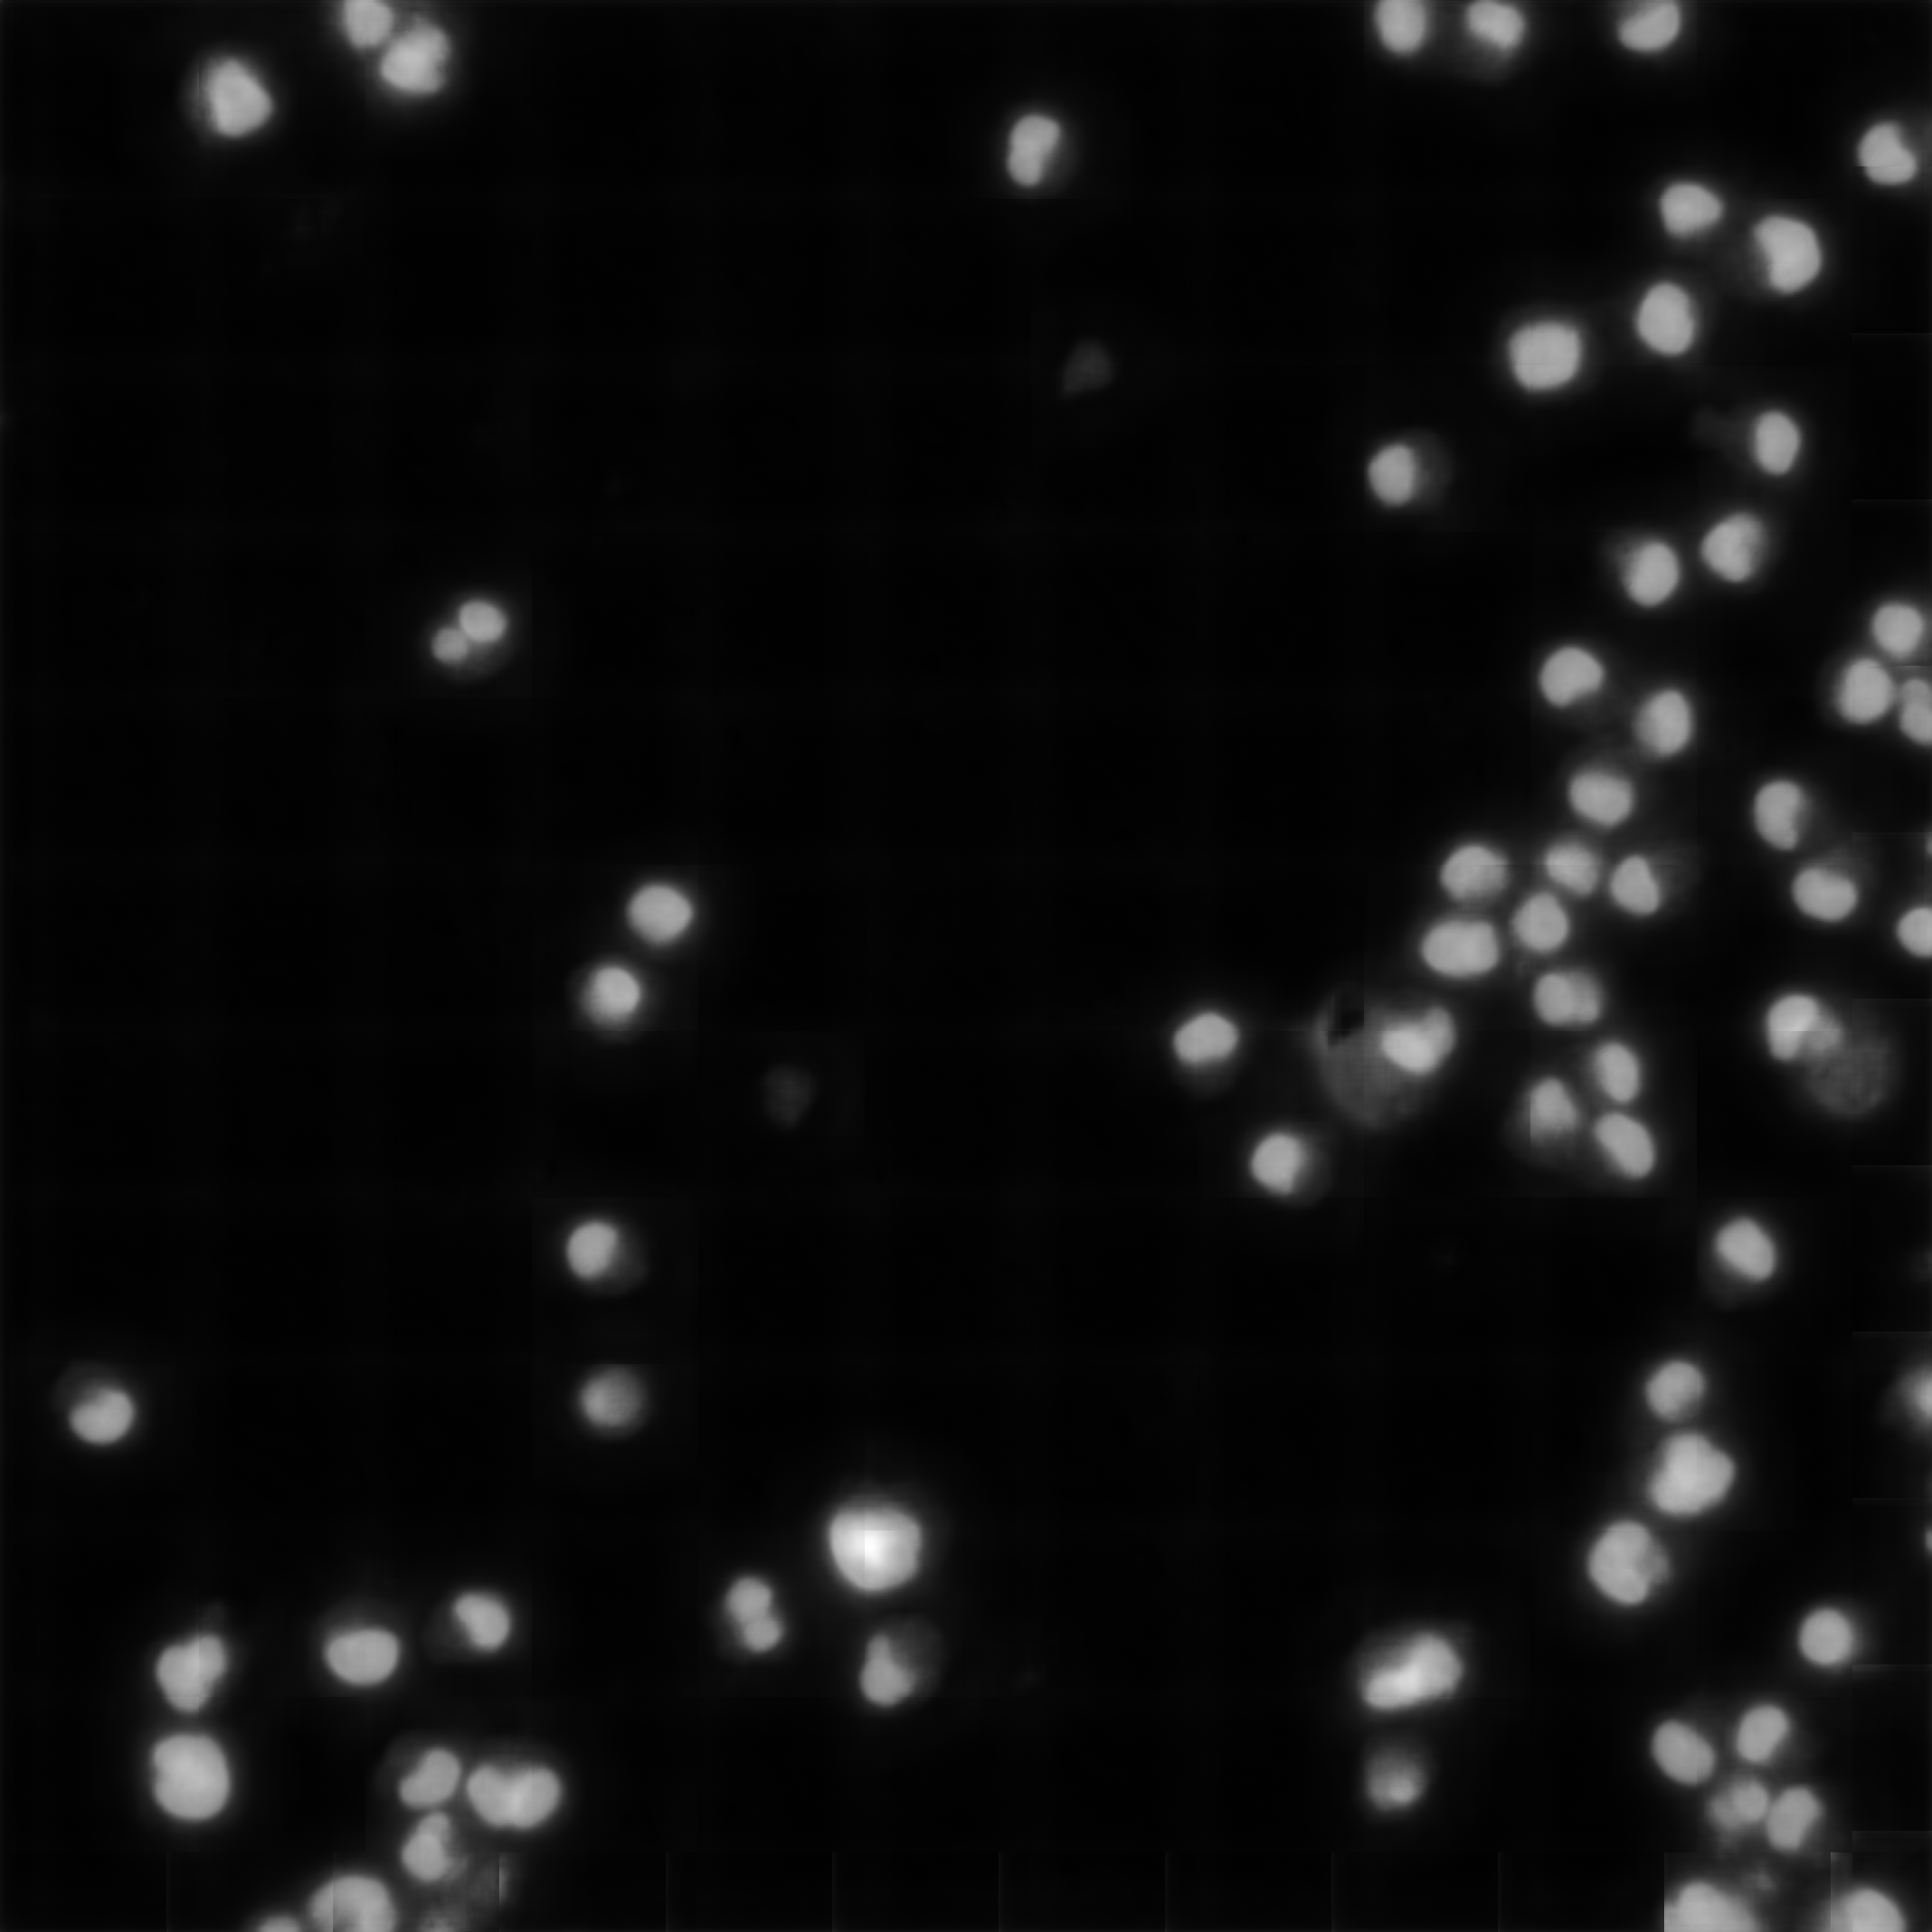
\includegraphics{bilder/lightning-conditions/lightning-1.png} & 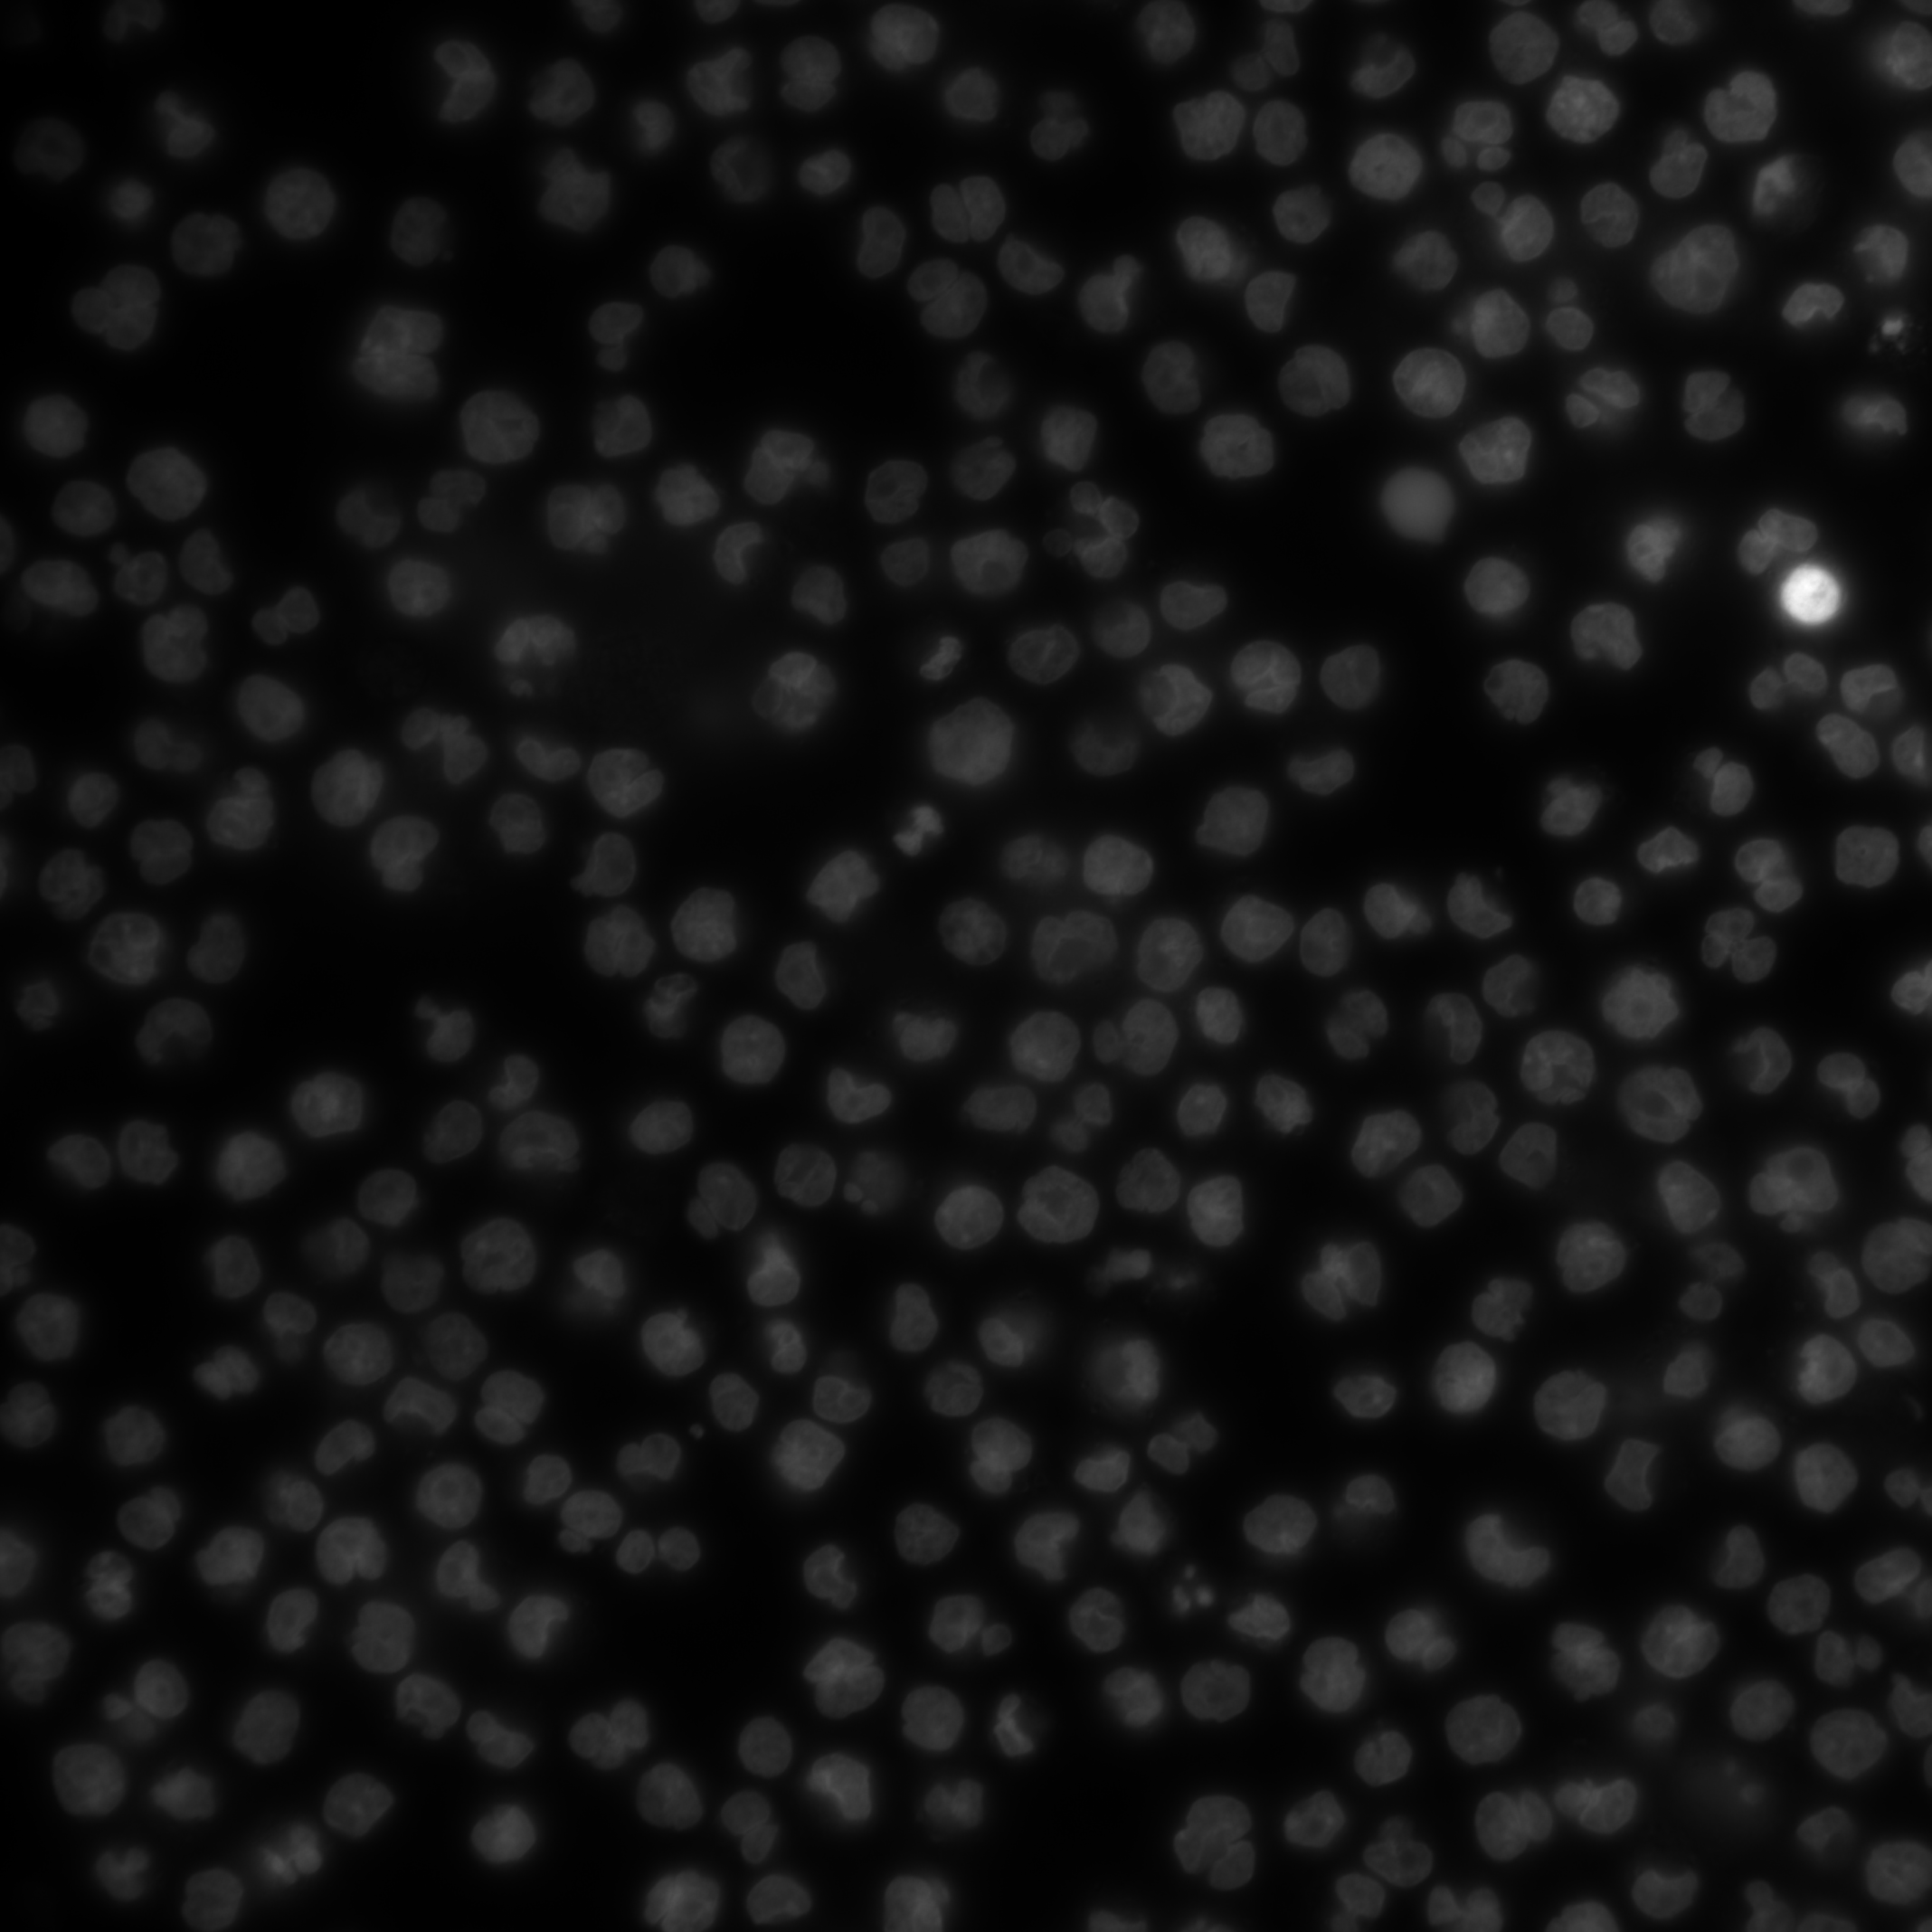
\includegraphics{bilder/lightning-conditions/lightning-2.png} &
            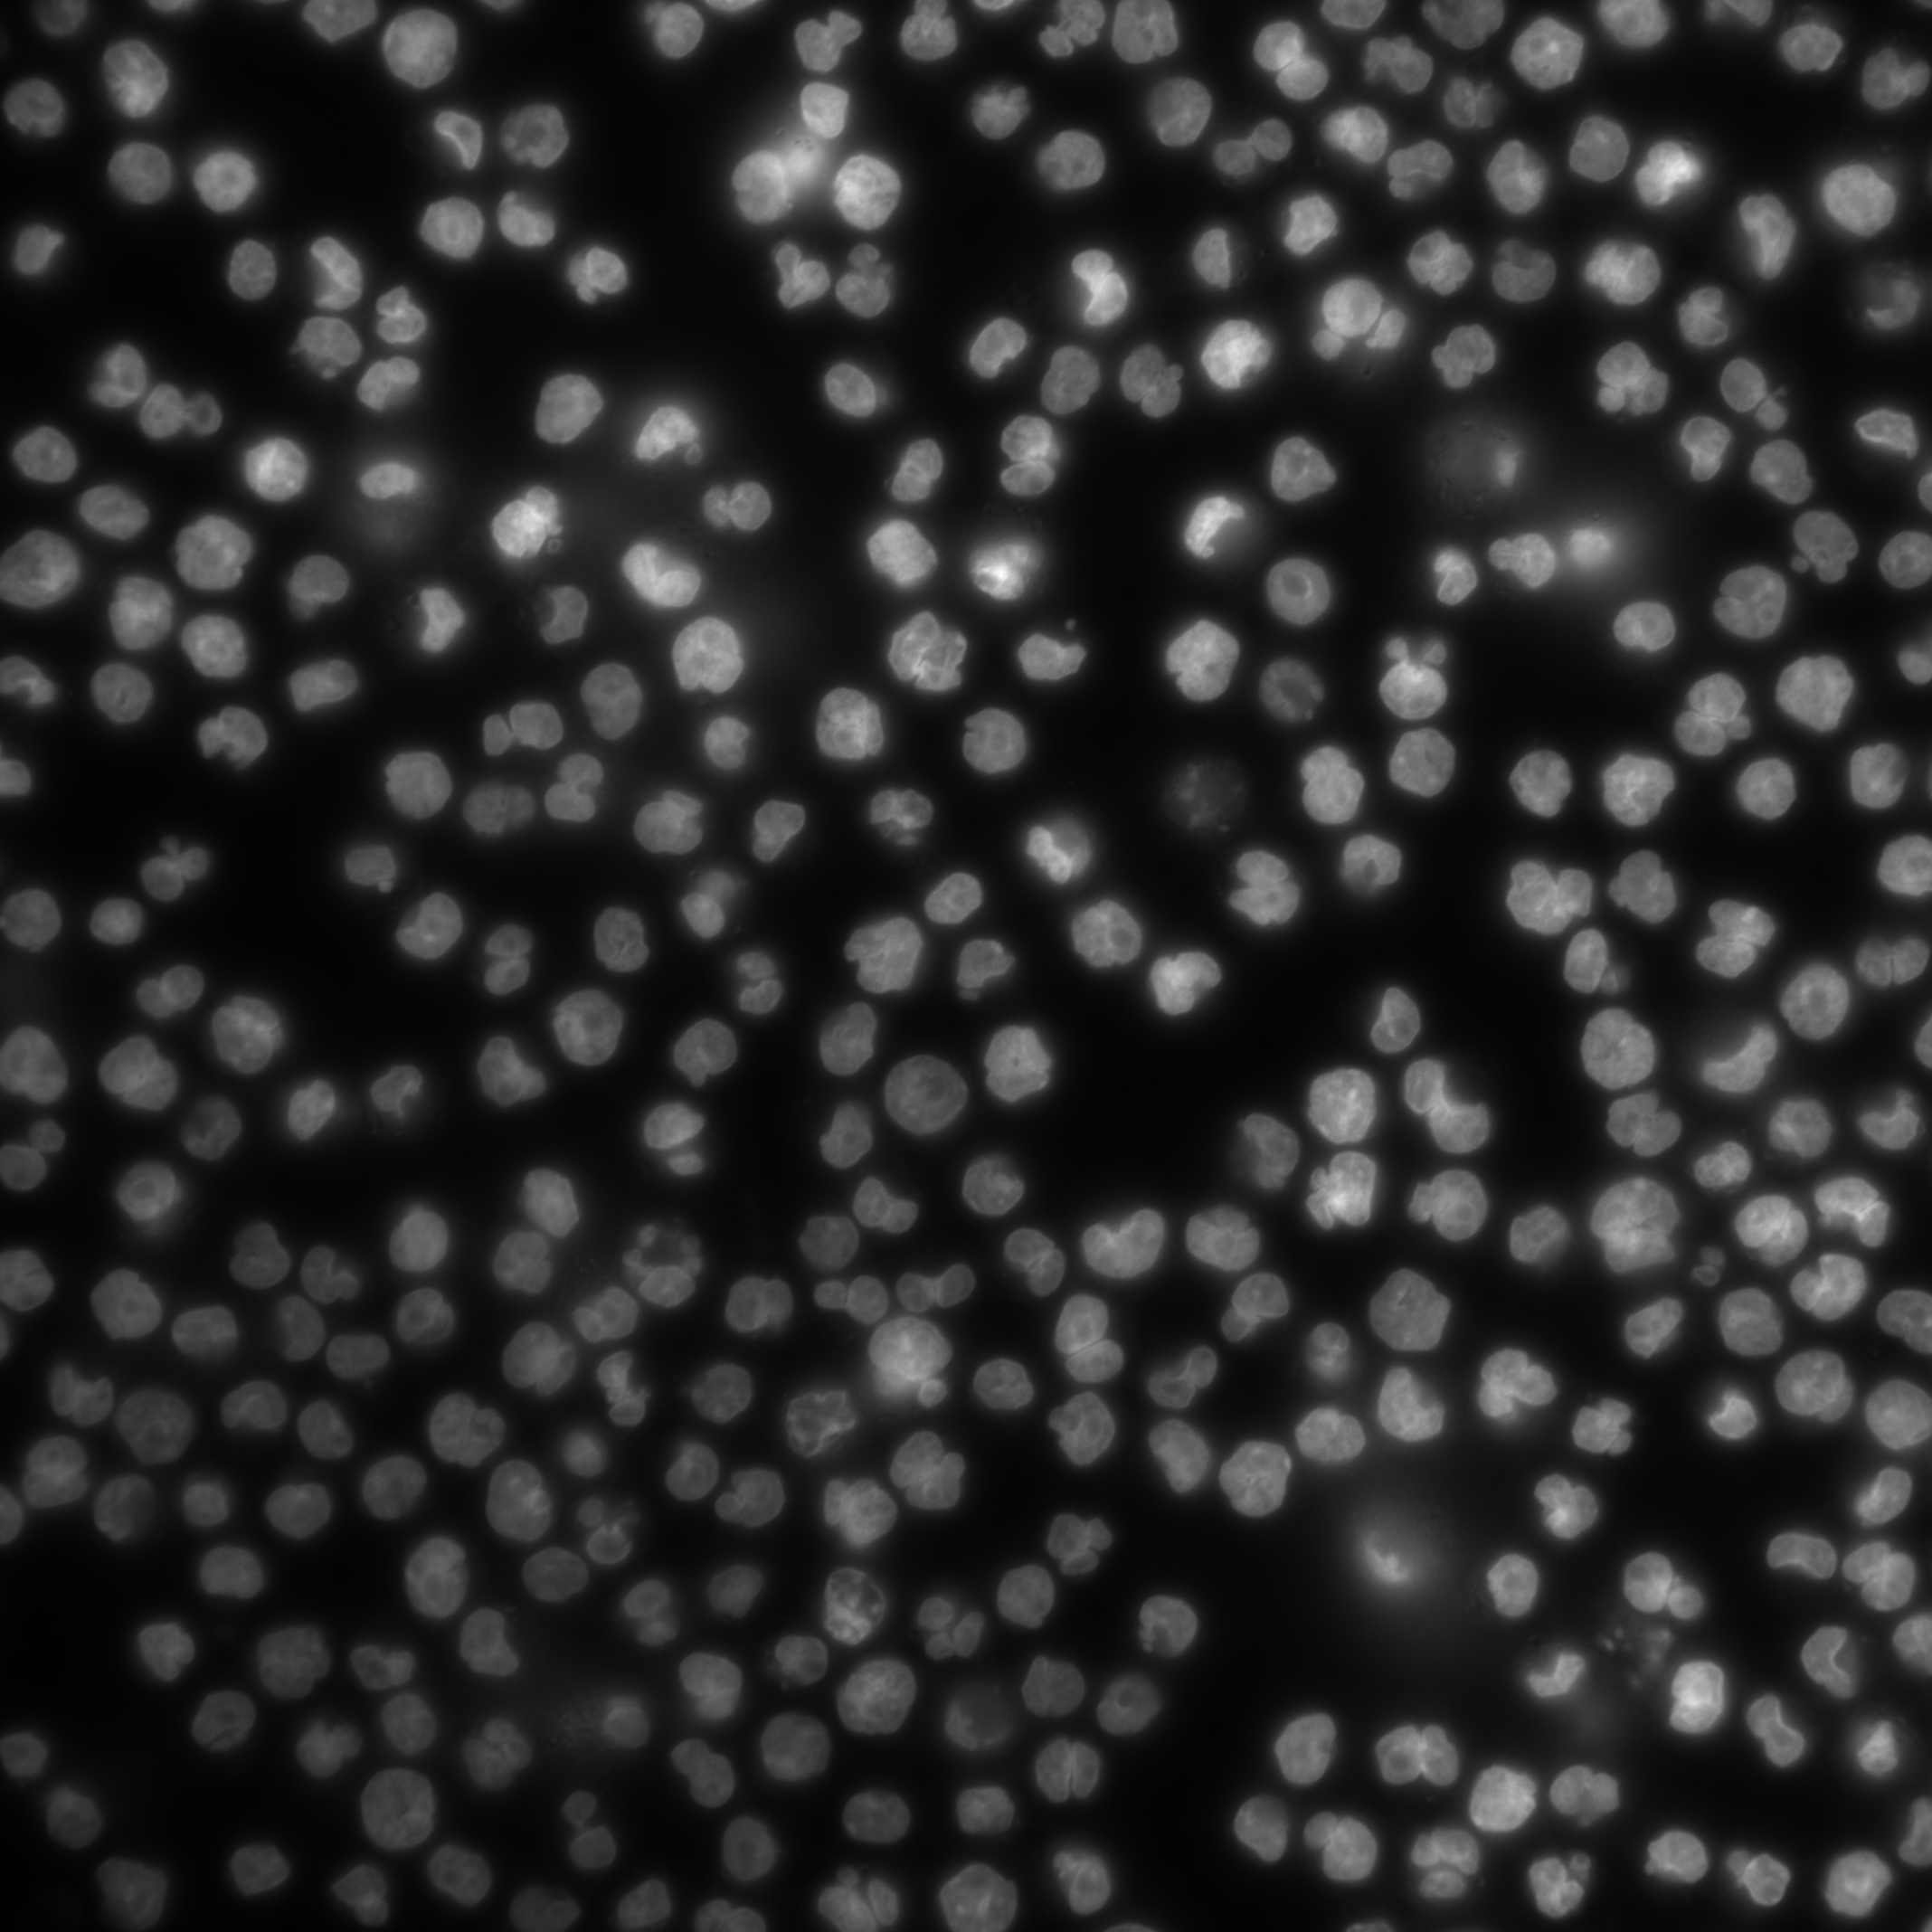
\includegraphics{bilder/lightning-conditions/lightning-3.png} & 
            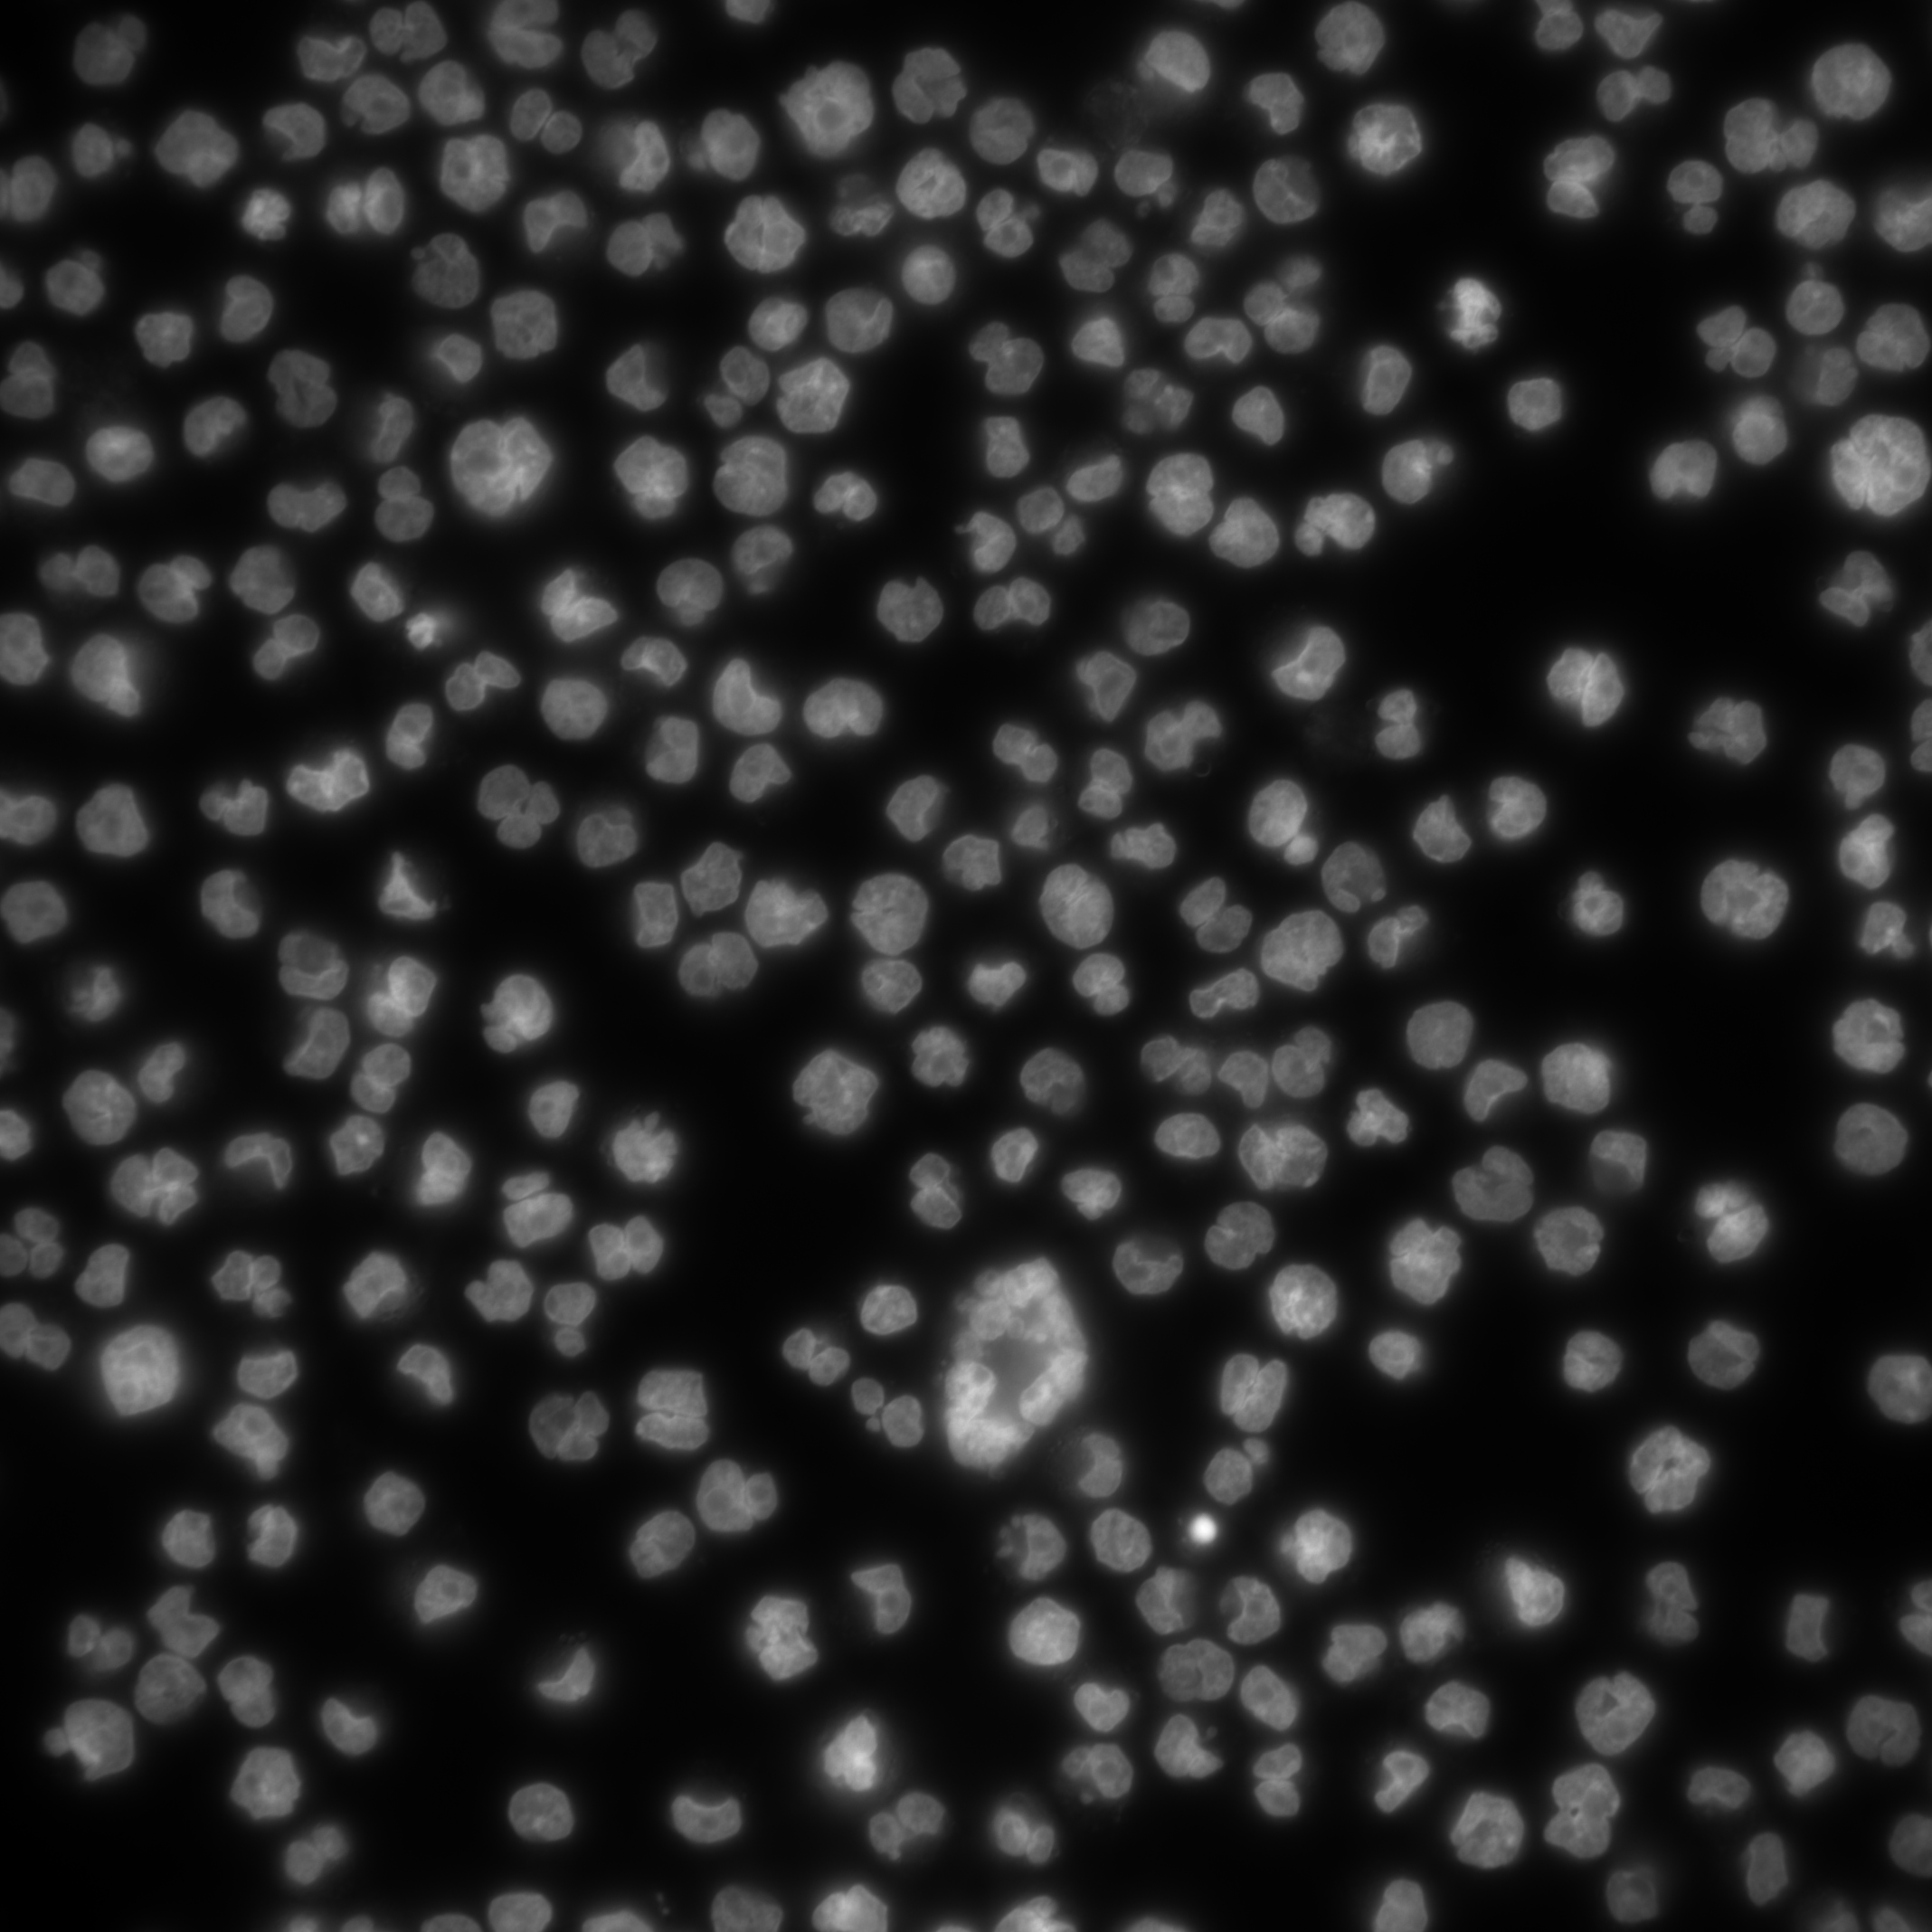
\includegraphics{bilder/lightning-conditions/lightning-4.png}
        \end{tabularx}
    \caption{Different lightning conditions}
    \label{fig:lightning_conditions}
\end{figure}